\documentclass{article}


% if you need to pass options to natbib, use, e.g.:
\PassOptionsToPackage{numbers, sort&compress}{natbib}
% before loading neurips_2022


% ready for submission
\usepackage{neurips_2022}

% to compile a preprint version, e.g., for submission to arXiv, add add the
% [preprint] option:
%     \usepackage[preprint]{neurips_2022}


% to compile a camera-ready version, add the [final] option, e.g.:
%     \usepackage[final]{neurips_2022}


% to avoid loading the natbib package, add option nonatbib:
% \usepackage[nonatbib]{neurips_2022}


\usepackage[utf8]{inputenc} % allow utf-8 input
\usepackage[T1]{fontenc}    % use 8-bit T1 fonts
\usepackage{hyperref}
% \usepackage{subfigure}
\usepackage{graphicx}    % hyperlinks
\usepackage{url}            % simple URL typesetting
\usepackage{color}
\usepackage{booktabs}       % professional-quality tables
\usepackage{amsfonts}       % blackboard math symbols
\usepackage{nicefrac}       % compact symbols for 1/2, etc.
\usepackage{microtype}      % microtypography
\usepackage{xcolor}         % colors
\usepackage{wrapfig}


\usepackage{times}
\usepackage{epsfig}
\usepackage{amsmath}
\usepackage{amssymb}

% Include other packages here, before hyperref.
\usepackage{float}
\usepackage{bbding}
\usepackage{pifont}
\usepackage{wasysym}
\usepackage{multirow}
\usepackage{subfig}



\title{Spatial-then-Temporal Self-Supervised Learning for Video Correspondence}


% The \author macro works with any number of authors. There are two commands
% used to separate the names and addresses of multiple authors: \And and \AND.
%
% Using \And between authors leaves it to LaTeX to determine where to break the
% lines. Using \AND forces a line break at that point. So, if LaTeX puts 3 of 4
% authors names on the first line, and the last on the second line, try using
% \AND instead of \And before the third author name.

\author{%
  David S.~Hippocampus\thanks{Use footnote for providing further information
    about author (webpage, alternative address)---\emph{not} for acknowledging
    funding agencies.} \\
  Department of Computer Science\\
  Cranberry-Lemon University\\
  Pittsburgh, PA 15213 \\
  \texttt{hippo@cs.cranberry-lemon.edu} \\
  % examples of more authors
  % \And
  % Coauthor \\
  % Affiliation \\
  % Address \\
  % \texttt{email} \\
  % \AND
  % Coauthor \\
  % Affiliation \\
  % Address \\
  % \texttt{email} \\
  % \And
  % Coauthor \\
  % Affiliation \\
  % Address \\
  % \texttt{email} \\
  % \And
  % Coauthor \\
  % Affiliation \\
  % Address \\
  % \texttt{email} \\
}


\begin{document}


\maketitle


\begin{abstract}
  Learning temporal correspondence from unlabeled videos is of vital importance in computer vision, and has been tackled by different kinds of self-supervised pretext tasks. For the self-supervised learning, recent studies suggest using large-scale video datasets despite the training cost. We propose a spatial-then-temporal pretext task to address the training data cost problem. The task consists of two steps. First, we use contrastive learning from unlabeled still image data to obtain appearance sensitive features. Then we switch to unlabeled video data and learn motion sensitive features by reconstructing frames. In the second step, we propose a global correlation distillation loss to retain the appearance sensitivity learned in the first step, as well as a local correlation distillation loss in a pyramid structure to combat temporal discontinuity. Experimental results demonstrate that our method surpasses the state-of-the-art self-supervised methods on a series of correspondence-based tasks. The conducted ablation studies verify the effectiveness of the proposed method.
\end{abstract}



\section{Introduction}
Learning representations for video correspondence is a fundamental problem in computer vision, which is closely related to different video applications, including optical flow estimation~\cite{dosovitskiy2015flownet}\cite{horn1981determining}, video object segmentation~\cite{caelles2017one}\cite{oh2019video}, keypoint tracking~\cite{xiu2018pose}, etc. However, supervising such a representation requires a large number of dense annotations, which is unaffordable. Thus most approaches acquire supervision from simulations~\cite{dosovitskiy2015flownet}\cite{mayer2016large} or limited annotations~\cite{pont20172017}\cite{xu2018youtube}, which result in poor generalization in different downstream tasks. Recently, self-supervised feature learning is gaining significant momentum, and several pretext tasks~\cite{jabri2020space}\cite{lai2020mast}\cite{li2019joint}\cite{wang2019learning}\cite{xu2021rethinking} are designed for space-time visual correspondence using large scale video datasets.
\vspace{-1mm}

The key to this task lies in two different perspectives. The first one is \textbf{temporal feature learning}, which aims to learn the fine-grained correspondence, i.e., motion between video frames. With the nature of temporal coherence in the video, the temporal feature learning can be formed as a reconstruction task, where the query pixel in the target frame can be reconstructed by leveraging the information of adjacent reference frames with a local range. Then a reconstruction loss is applied to minimize the photometric error between the raw frame and its reconstruction. However, the temporal discontinuity occurs frequently due to the occlusions, dramatic appearance changes, and deformations, especially for pixels in each frame with large down-sampling. In such scenarios, the frame reconstruction loss apparently becomes invalid, which results in inferior performance. To alleviate the problem, MAST~\cite{lai2020mast} applies frame reconstruction with a higher feature resolution by decreasing the stride of the backbone, which requires a larger memory and computation cost. Another way to utilize free temporal supervision is by exploiting temporal cycle-consistency.  \cite{jabri2020space}\cite{wang2019learning} track objects forward and backward with the objective of maximizing the cycle-consistency using  reconstruction and contrastive loss. Compared to the correspondence learning realized at object-level, the frame reconstruction is conducted on raw image space, which provides more accurate supervision for learning fine-grained correspondence.

\begin{figure}[!tb]
  \centering
  {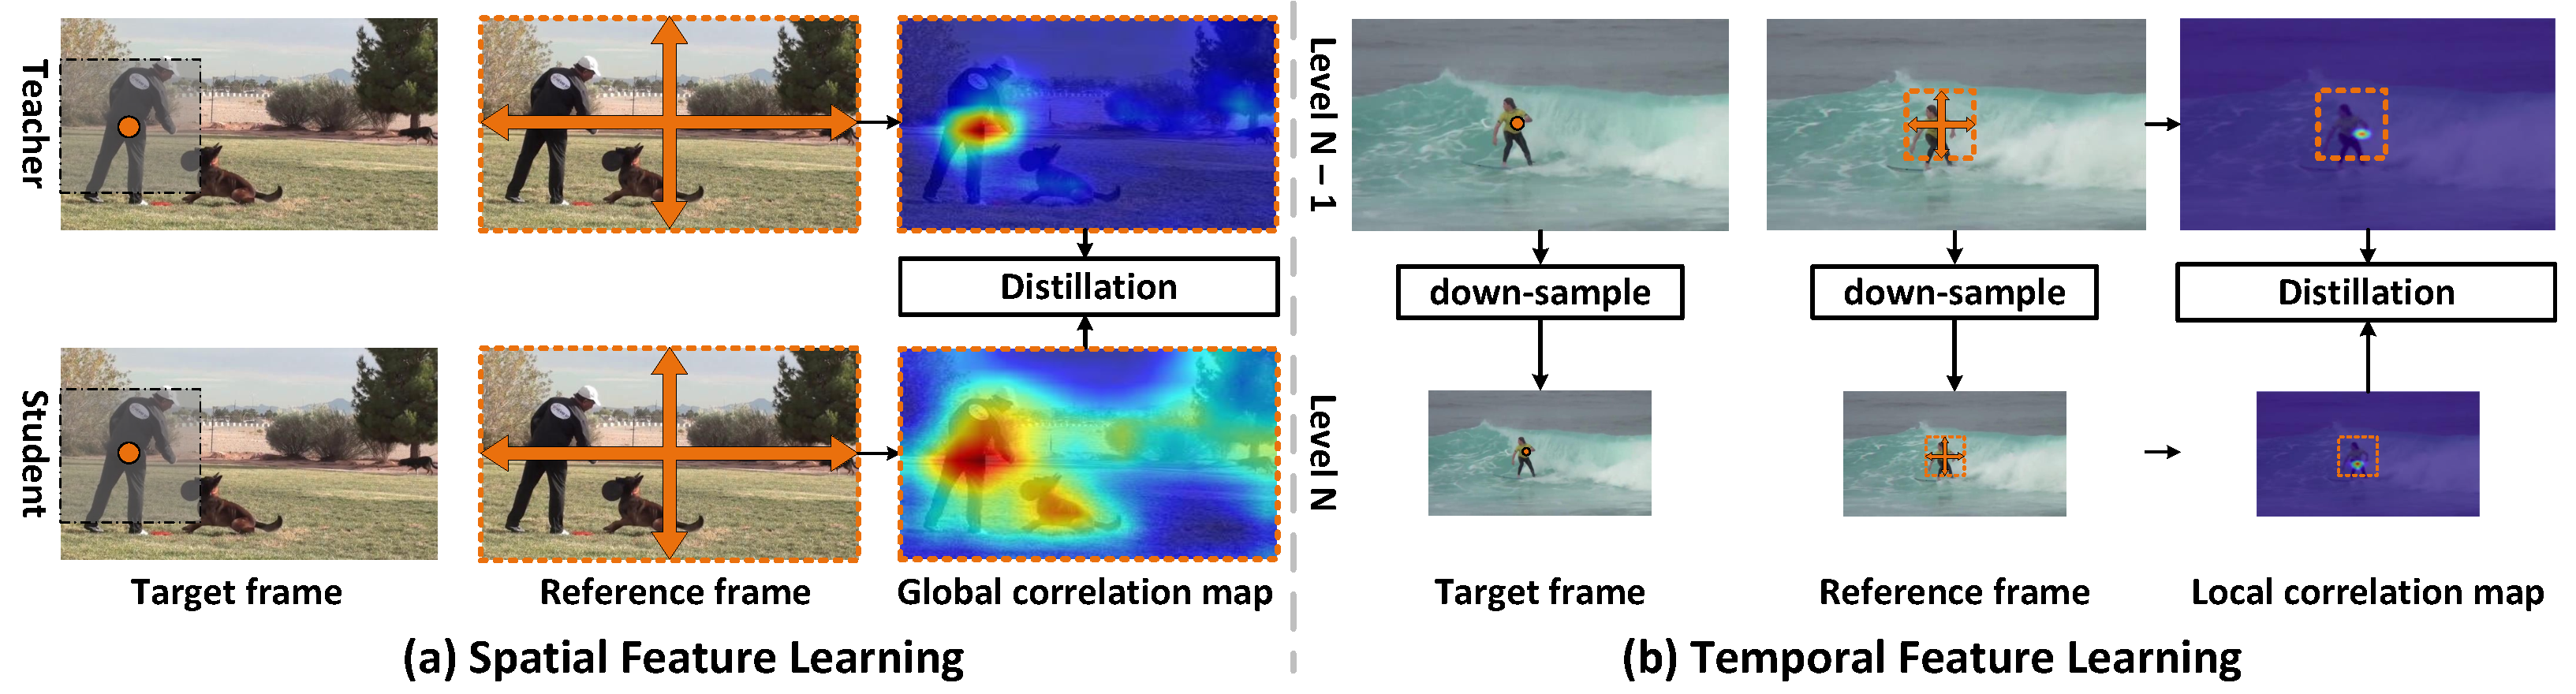
\includegraphics[width=1.0\textwidth]{figure/tissor/tissor.pdf}}
  \caption{\small \textbf{Illustration of the main idea.} In (a), we first train a contrastive model on image data and fix it as teacher. Then the distillation on global correlation maps is proposed to retain appearance sensitivity. In (b), the distillation is performed between local correlation maps at different pyramid levels to facilitate fine-grained matching. The local correlation map computed at lower pyramid level is regarded as pseudo labels. The dashed line with cross in orange represents the range of computing correlation map w.r.t. query point.}
  \label{fig:tissor}
  \vspace{-7mm}
\end{figure}

The second one is \textbf{spatial feature learning}. Spatial feature learning aims to learn the object appearance that is invariant to viewpoint and appearance changes, thus providing temporal correspondence with robust appearance cues especially when facing temporal  discontinuity. \cite{wang2020contrastive} adopts a intra-inter consistency loss to learn  discriminative spatial feature while \cite{xu2021rethinking} learns the space-time correspondence through a frame-wise contrastive loss. Both methods are trained on large-scale video datasets and try to realize the spatial and temporal feature learning in a unified framework, which is sub-optimal for each of them. Recently, as mentioned in~\cite{wang2021different}, the contrastive model~\cite{he2020momentum}\cite{xie2021detco} pre-trained on image data shows competitive performance against dedicated methods for video correspondence due to its superior capability of learning spatial representation. However, such a model still fails to realize the fine-grained matching between video frames. This motivates us to design a framework that subsequently learns the motion sensitive features with video data.

In this paper, we propose a spatial-then-temporal pretext task, which decouples self-supervised video correspondence learning into two steps, including spatial and temporal feature learning. To achieve this, we first train the model in a contrastive learning paradigm with unlabeled image data~\cite{deng2009imagenet} which has a much smaller data size than video~(see Table~\ref{table:sota}), e.g., Kinetics~\cite{carreira2017quo}, TrackingNet~\cite{muller2018trackingnet}, in order to learn appearance sensitive features. Then, we perform the temporal feature learning on a small video dataset~\cite{xu2018youtube}.  However, directly fine-tuning the old model with only new data will lead to a well-known phenomenon of catastrophic forgetting~\cite{li2017learning}. To address this problem, as shown in Figure \ref{fig:tissor} (a), we freeze the model pre-trained in the first stage  as teacher. Then a global correlation distillation loss is proposed to retain the appearance sensitive features. At the same time, we propose a pyramid learning framework to combat severe information loss and temporal discontinuity due to spatial down-sampling. First, the frame reconstruction is applied at different levels of the network to better exploit the fine-grained temporal supervision. As observed in Figure \ref{fig:tissor} (b), the pixels of the target and reference frame with higher resolution have a lower chance of facing temporal discontinuity, which provides a more accurate local correlation map. Thus we design a local correlation distillation loss that supports explicitly learning of the correlation map in the region with high uncertainty, which is achieved by taking the finest local correlation map as pseudo labels. 

To sum up, our main contributions include: (a) We propose a novel spatial-then-temporal pretext task for self-supervised video correspondence, which addresses the training data cost problem by learning appearance and motion sensitive features sequentially. (b) We introduce a global correlation distillation loss to retain the appearance sensitivity learned in the first step when training on a video dataset. (c) We propose a local correlation distillation loss to combat the temporal discontinuity of frame reconstruction in the region with high uncertainty.  (d) We verify our approach in a series of correspondence-related tasks, including video object segmentation, human parts propagation, and pose tracking. Our approach consistently outperforms previous state-of-the-art self-supervised methods and is even comparable with some task-specific fully-supervised algorithms.
\vspace{-4mm}

\section{Related Work}
\textbf{Self-supervised learning for video correspondence.} 
Recent approaches focus on learning correspondence from unlabeled videos in a self-supervised manner. The task requires the model to have the ability to capture object appearance and estimate the motion between frames at the same time, which has proceeded along two different dimensions: reconstruction-based methods~\cite{lai2019self}\cite{lai2020mast}\cite{li2019joint}\cite{vondrick2018tracking}\cite{wang2020contrastive} and cycle-consistency-based methods \cite{jabri2020space}\cite{wang2019learning}\cite{zhao2021modelling}. In the first type, a query point is reconstructed from adjacent frames while the latter performs forward-backward tracking with the objective of minimizing the cycle inconsistency. Through getting promising results, most methods address the problem by considering only one perspective. VFS~\cite{xu2021rethinking} learns the spatial and temporal representation through a frame-wise contrastive loss while~\cite{araslanov2021dense}\cite{wang2020contrastive} try to realize the spatial and temporal feature learning in a unified framework by exploiting the inter-video constraint, which may result in sub-optimal performance. In this paper, we learn a better representation by proposing a spatial-then-temporal pretext task, which learns appearance and motion sensitive features sequentially.


\textbf{Self-supervised spatial feature learning.} Self-supervised spatial feature learning aims to learn discriminative features of object appearance with unlabeled data, which recently gets promising result with contrastive learning. In an early work~\cite{wu2018unsupervised}, the contrastive learning is formulated as an instance discrimination task, which requires the model to return low values for similar pairs and high values for dissimilar pairs. Recently, the performance is further improved by creating a dynamic memory-bank~\cite{he2020momentum}, introducing online clustering~\cite{caron2020unsupervised} and avoiding the use of negative pairs~\cite{chen2021exploring}\cite{grill2020bootstrap}. Furthermore, \cite{wang2021dense}\cite{xie2021detco}\cite{yang2021instance} propose various pretext tasks to adapt the contrastive learning to dense prediction tasks. Even though showing superior performance for temporal correspondence~\cite{wang2021different}, the contrastive model pre-trained on image data still struggles to model the motion between video frames. 

\textbf{Self-supervised temporal feature learning. } 
Compared to spatial feature learning, temporal feature learning focus on learning the motion information of video, which is closely related to optical flow and motion estimation. Most methods~\cite{dosovitskiy2015flownet}\cite{teed2020raft} directly regress the ground-truth optical flow produced by synthetic datasets, thus suffering from severe domain shift. To deal with the problem, \cite{meister2018unflow} tries to learn the dense correspondence on real video without any label by minimizing the photometric error between the raw frame and its reconstruction in the valid region. However, the video frames usually contain temporal discontinuity including dramatic appearance changes and occlusions, which seriously degrades the capability of the method. \cite{jonschkowski2020matters}\cite{liu2020learning}\cite{liu2019ddflow} alleviate the problem by utilizing the optical flow predictions from teacher model to guide the learning of student model. In this paper, we address the issue by: (1)~learning object representation that is invariant to appearance changes with contrastive learning. (2)~proposing a local correlation distillation loss in a pyramid structure. 


\section{Approach}
The basic idea of our method is to decouple video correspondence learning into two  steps, including spatial and temporal feature learning. We first train our model using contrastive loss with still image data to learn appearance sensitive features. Then, we perform the temporal feature learning on a small video dataset to learn the fine-grained correspondence between frames. In the second step, we propose a global correlation distillation loss to retain the ability to capture object appearance while address the problem of temporal discontinuity by introducing a local correlation distillation loss with a pyramid learning framework.

\begin{figure}[!tb]
  \centering
  {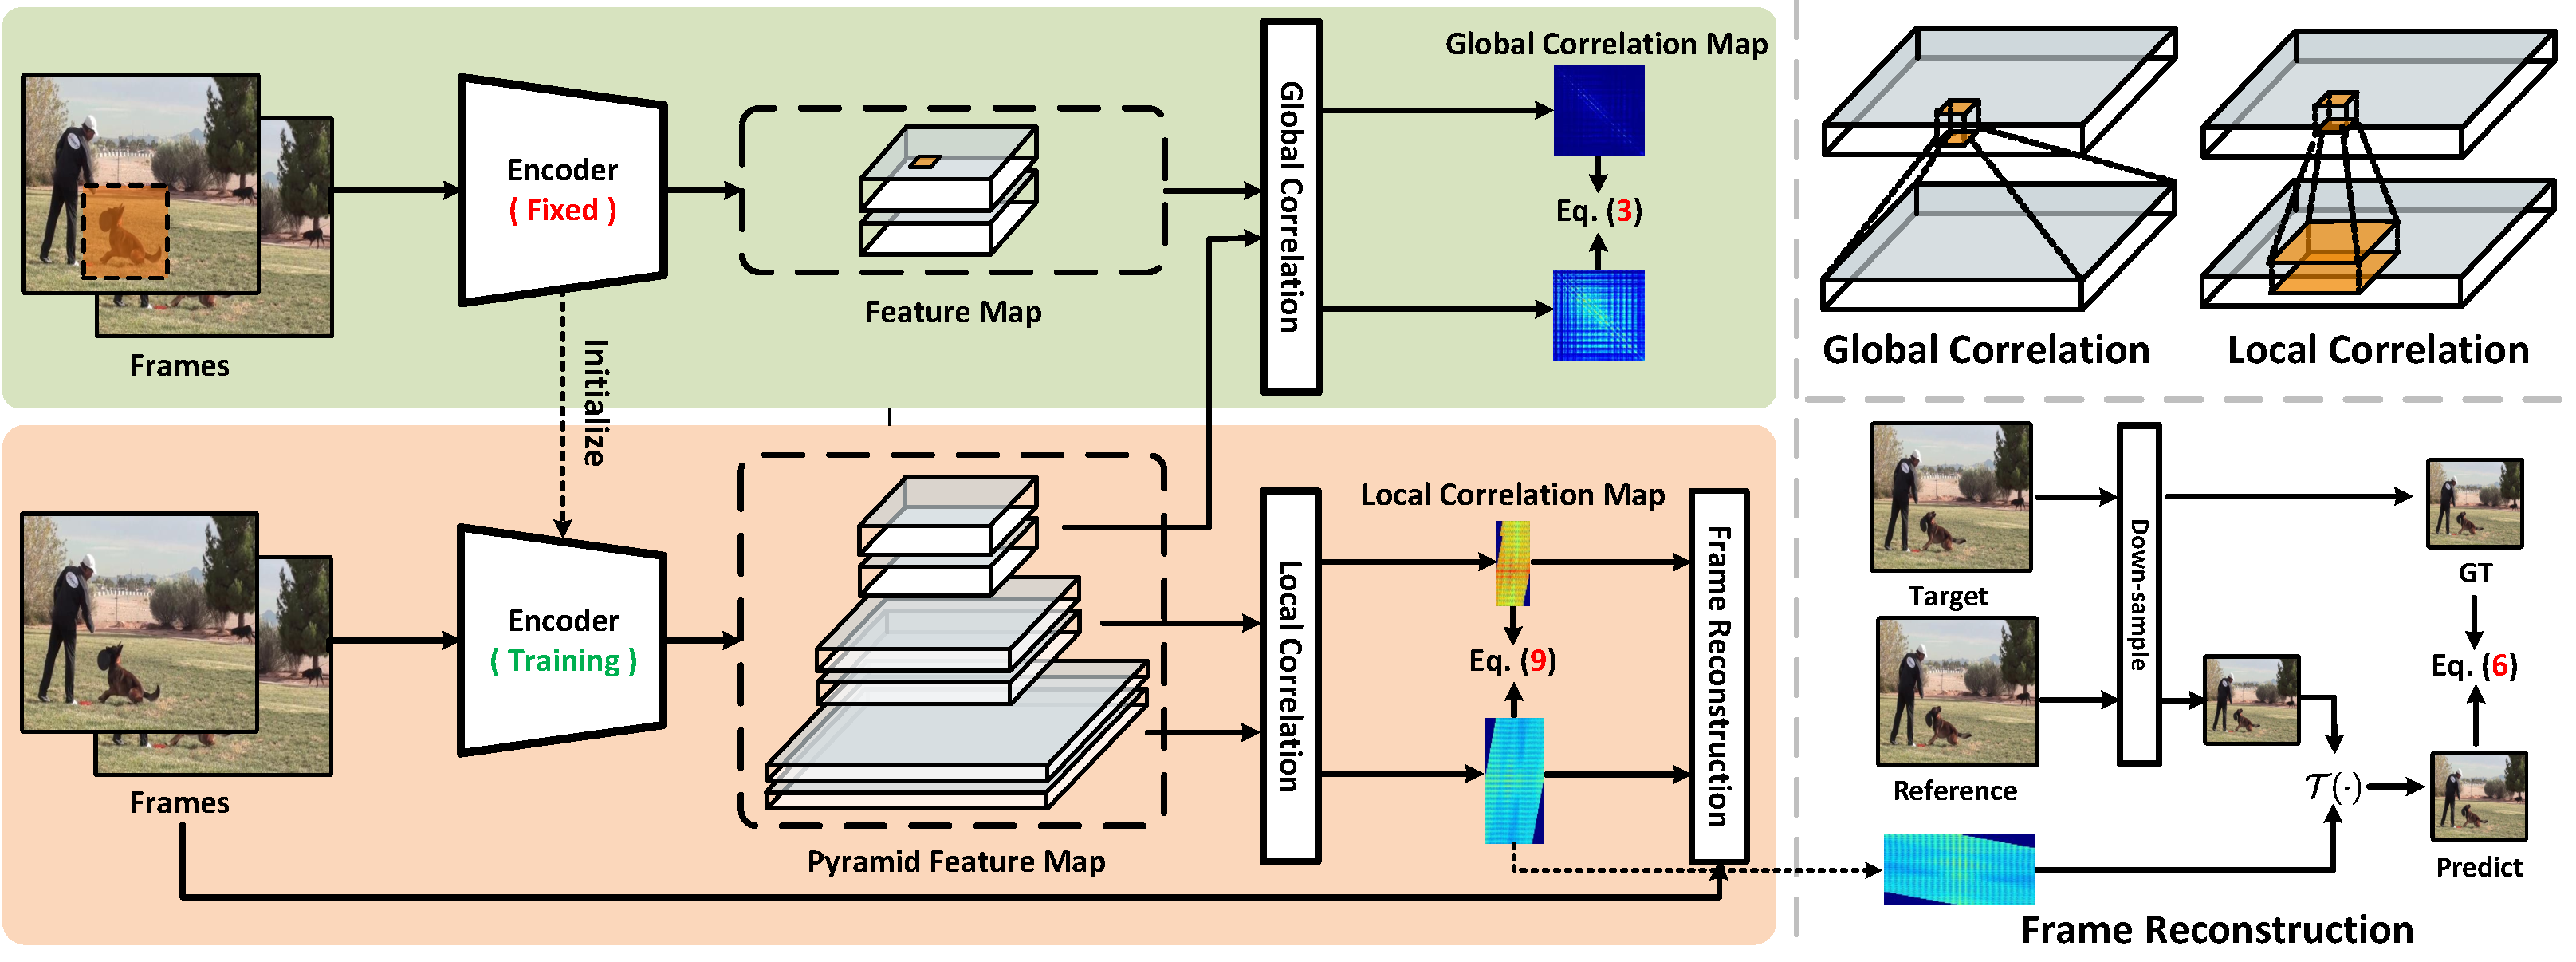
\includegraphics[width=1.0\textwidth]{figure/framework/framework.pdf}}
  \caption{\small \textbf{Overview of the second step in our pretext task. The fixed encoder was trained in the first step (not shown).} We first exploit the contrastive loss to learn the appearance sensitive features with still image data (not shown). Then we perform the temporal feature learning with video data in the second step. To retain the appearance sensitivity, we fix the pre-trained network as teacher and a global correlation distillation loss is devised between global correlation maps. To address the issue of temporal discontinuity, we first apply frame reconstruction at each pyramid level of the network. Then the distillation is conducted between local correlation maps computed at different pyramid levels, which learns better motion sensitive features by taking fine-grained local correlation maps as pseudo labels. }
  \label{fig:framework}
  \vspace{-5mm}
\end{figure}

\subsection{Spatial Feature Learning}
\label{spatial_feature_learning}
The spatial feature mainly describes the appearance of objects involved in an image. Spatial feature learning is analogous to that of instance discrimination and thus easily benefits from the recent advancements brought by contrastive learning. We first briefly review the instance discrimination objective in contrastive learning. Given an encoded query $\boldsymbol{q}\in\mathbb{R}^d$ and a set of encoded key vectors $\mathcal{K}=\left\{\boldsymbol{k}^{+}, \boldsymbol{k}_{1}^{-}, \boldsymbol{k}_{2}^{-}, \ldots, \boldsymbol{k}_{K}^{-}\right\}$ which consists of one positive key $\boldsymbol{k}^{+}\in\mathbb{R}^d$ and $K$ negative keys $\mathcal{K^{-}}=\left\{\boldsymbol{k}_{j}^{-}\right\}$, where $d$ denotes the embedding dimension. The query and its positive key are generated from the same instance with two different augmentations, while the negative keys refer to other instances. The objective of instance discrimination is to maximize the similarity between the query $\boldsymbol{q}$ and the positive key $\boldsymbol{k}^{+}$ while remaining query distinct to all negative keys $\mathcal{K^{-}}$. Thus, a contrastive loss is presented in InfoNCE~\cite{van2018representation}  with a softmax formulation:
	\begin{equation}\label{eq:nce}
		\small
		\begin{aligned}
			\mathcal{L}_{\text{nce}}=-\log \frac{\exp \left(\boldsymbol{q}^{T} \boldsymbol{k}^{+} / \tau_c\right)}{\exp \left(\boldsymbol{q}^{T} \boldsymbol{k}^{+} / \tau_c\right)+\sum_{i=1}^{K} \exp \left(\boldsymbol{q}^{T} \boldsymbol{k}_{i}^{-} / \tau_c\right)}
		\end{aligned}~~,
	\end{equation}
where the similarity is measured via dot product, and $\tau_c$ is the temperature hyper-parameter. MoCo~\cite{he2020momentum} builds a dynamic memory bank to maintain a large number of negative samples with a moving-averaged encoder. DetCo~\cite{xie2021detco} further improves the contrastive loss $\mathcal{L}_{\text{nce}}$ by introducing a global and local contrastive learning to enhance local representation for dense prediction. In this paper, we adopt the same framework as~\cite{he2020momentum}\cite{xie2021detco} to learn an appearance model for most of our experiments.

\textbf{Global correlation distillation.} After training with contrastive loss, we get an encoder $\phi$. Then we continuously train it on video data to learn the fine-grained correspondence (See section \ref{temporal_feature_learning}). However, directly fine-tuning the old model with only new data will lead to a well-known phenomenon of catastrophic forgetting~\cite{li2017learning}, which degrades the performance. Thus we introduce a global correlation distillation loss in order to retain the ability to capture object appearance. More specifically, we first fix the feature encoder $\phi$ as teacher denoted as $\phi_t$. Given a pair of video frames consisting of target and reference frame $I_{t}, I_r$, the  $\phi$ maps them to a pair of feature embeddings $F^l_t,F^l_{r} \in \mathbb{R}^{h^l w^l \times d^l}$, where $l \in \{0, 1, \ldots, N \}$ is the index of each pyramid level and the bigger number represents the coarser pyramid level. For each query point $F^N_t(i)$ and key point $F^N_r(j)$ at pyramid level $N$, we compute the global correlation $a^N_{i, j}$ using a softmax over similarities w.r.t. all keys in the reference frame (see the upper right of Figure \ref{fig:framework}), i.e.
\begin{equation}\label{eq:global_correlation}
  \small
  \begin{aligned}
    a^N_{i, j}=\frac{\exp \left(F^N_t(i)  \cdot F^N_r(j) / \tau\right)}{\sum_{n} \exp \left(F^N_t(i) \cdot F^N_r(n) / \tau\right)}, i,j,n \in \{1,\ldots,h^Nw^N\}
  \end{aligned}~~,
\end{equation}
Where ‘·’ stands for the dot product. Each point in $F^N_t$ and $F^N_{r}$ covers a relatively large region since the output stride is set to 32 in our feature encoder. Thus, we can form the global correlation as object-level correspondence, which is closely related to object appearance. We generate the pseudo labels $\hat{a}^N$  using Eq \ref{eq:global_correlation} with $\phi_t$. The global correlation distillation loss $\mathcal{L}_{\mathrm{gc}}$ is defined to minimize the mean squared error between $a^N$ and $\hat{a}^N$.
\begin{equation}\label{eq:global_correlation_loss}
  \small
  \begin{aligned}
    % \mathcal{L}_{gc}  =\sum_{i}\sum_{j} \left\|a_{i,j}-a^t_{i,j}\right\|_{2}^{2}
    \mathcal{L}_{\mathrm{gc}}  = \left\|a^N-\hat{a}^N\right\|_{2}^{2}
  \end{aligned}~~,
\end{equation}
\subsection{Temporal Feature Learning}
\label{temporal_feature_learning}
We then perform temporal feature learning right after spatial feature learning. Temporal feature learning aims to learn the fine-grained correspondence between video frames. Recently, a few studies~\cite{lai2020mast}\cite{vondrick2018tracking} introduce a reconstruction-based correspondence learning scheme, where each query pixel in the target frame can be reconstructed by leveraging the information of adjacent reference frames with a limited range. More specifically, the target and reference frame $I_{t}, I_r$ are projected into a  fine-grained pixel embedding space. We denoted these embedding as $F_t,F_{r} \in \mathbb{R}^{hw \times d}$. For each query pixel $i$ in $I_{t}$, we can calculate the local correlation $c_{i,j}$ w.r.t. the reference frame in a local range~(see the upper right of Figure \ref{fig:framework}):
\begin{equation}\label{eq:local_correlation}
  \small
  \begin{aligned}
    c_{i, j}=\frac{\exp \left(F_t(i)  \cdot F_r(j) / \tau\right)}{\sum_{n} \exp \left(F_t(i) \cdot F_r(n) / \tau\right)}, i \in \{1,\ldots,hw\}, j,n \in \mathcal{N}(i)
  \end{aligned}~~,
\end{equation}
Where $\mathcal{N}(i)$ is the index set with a limited range of $r$ pixels for pixel $i$. Then each query pixel $i$ in target frame can be reconstructed by a weighted-sum of pixels in $\mathcal{N}(i)$, according the local correlation map $c \in \mathbb{R}^{hw \times (r)^2}$:
\begin{equation}\label{eq:reconstruction}
  \small
  \begin{aligned}
    \hat{I}_{t}(i)=\sum_{j \in \mathcal{N}(i)} c_{i,j} I_{r}(j)
  \end{aligned}~~,
\end{equation}
We regard the above process as a transformation function for all query pixels and denotes it as: $\hat{I}_{t} = \mathcal{T}\left(c, I_r\right)$. Then the reconstruction loss $\mathcal{L}_{\mathrm{rec}}$ is defined as L1 distance between $\hat{I}_{t}$ and $I_{t}$.
\begin{equation}\label{eq:reconstruction loss}
  \small
  \begin{aligned}
    \mathcal{L}_{\mathrm{rec}}=\left\|\hat{I}_{t} - I_{t}\right\|_{1}
  \end{aligned}~~,
\end{equation}
However, the Eq \ref{eq:reconstruction} should only be applied when the feature embedding has the same size as video frame. Thus the stride of $\phi$ must be set to 1, which introduces large memory and computation cost. One possible solution is to apply down-sampling on the target and reference frame. MAST~\cite{lai2020mast} proposes an image feature alignment module that samples the pixel at the center of strided convolution kernels. However, down-sampling with a large rate would cause severe information loss and result in more pixel occlusions between video frames, which obviously degrades the representation of temporal feature learning. To address the issue, we design a pyramid learning framework consisting of pyramid frame reconstruction and local correlation distillation with entropy-based selection.

\textbf{Pyramid frame reconstruction.}  As observed in Figure \ref{fig:framework}, we obtain a pair of feature pyramids $\{F^l_t\}^{N-1}_{l=1}$,$\{F^l_{r}\}^{N-1}_{l=1}$.  Then we get the pyramid local corelation map $\{c^l\}^{N-1}_{l=1}$ at each pyramid level by utilizing Eq \ref{eq:local_correlation} with different range $r^l$. As the same time, we adopt a same down-sampling method as~\cite{lai2020mast} to get a pair of frame pyramids $\{I^l_t\}^{N-1}_{l=1},\{I^l_{r}\}^{N-1}_{l=1}$, which has same shape with the feature pyramids at each pyramid level. Given the $c^l$, $I^l_t$ and $I^l_r$, we apply the pyramid reconstruction loss:
\begin{equation}\label{eq:pyramid reconstruction loss}
  \small
  \begin{aligned}
    \mathcal{L}^{p}_{\mathrm{rec}}=\sum_l\left\|\mathcal{T}\left(c^l, I^l_r\right) - I^l_{t}\right\|_{1}
  \end{aligned}~~,
\end{equation}
By doing this, we are able to exploit more fine-grained temporal supervision and get better temporal representation at the intermediate pyramid level. 

\textbf{Local correlation distillation.} The bottom level of the frame pyramid contains more fine-grained information and suffer less occlusions for temporal feature learning due to relatively small down-sampling rate, which may result in more accurate local correlation map. Inspired by it, we design a novel local correlation distillation loss which explicitly make constraint on the final local correlation map $c^{N-1} \in \mathbb{R}^{h^{N-1}w^{N-1} \times (r^{N-1})^2}$. We first compute the local correlation map $c^{N-2}$ at level $N-2$ and then apply  correlation down-sampling~\cite{teed2020raft} to get pseudo labels $\hat{c}^{N-1}$ with the same size as $c^{N-1}$.  Then the local correlation distillation loss $\mathcal{L}_{lc}$ is adopt to minimize the mean squared error between $c^{N-1}$ and $\hat{c}^{N-1}$.\\

\textbf{Entropy-based selection.} The correlation of each query w.r.t. reference frame indicates more uncertainty when having smooth distribution, which should be paid more attention to when applying distillation. Thus we calculate the entropy for each query $i$:
\begin{equation}\label{eq:pyramid reconstruction loss}
  \small
  \begin{aligned}
    \mathcal{H}(i)=\sum_j-log c^{N-1}_{i,j}
  \end{aligned}~~,
\end{equation}
Then we obtain a mask $m \in \mathbb{R}^{h^{N-1}w^{N-1}}$ to filter out the region with lower entropy by setting a threshold $T$. The local correlation distillation loss with entropy selection is defined as:
\begin{equation}\label{eq:reconstruction loss}
  \small
  \begin{aligned}
    \mathcal{L}^e_{\mathrm{lc}}=\sum_im_i\left\|c_{i,:}^{N-1}-\hat{c}^{N-1}_{i,:}\right\|^2_{2}
  \end{aligned}~~,
\end{equation}
Eventually, our training loss of temporal feature learning is defined as: $\mathcal{L}_\mathrm{t}$ =  $\mathcal{L}^p_{\mathrm{rec}} + \alpha  \mathcal{L}^e_{\mathrm{lc}}$. The final loss of training on video data is a weighted sum of  $\mathcal{L}_\mathrm{t}$ and a regularization term $\mathcal{L}_\mathrm{gc}$ introduced in Section \ref{spatial_feature_learning}:
\begin{equation}\label{eq:final loss}
  \small
  \begin{aligned}
    \mathcal{L} = \mathcal{L}_{\mathrm{t}}  + \beta  \mathcal{L}_{\mathrm{gc}}
  \end{aligned}~~,
\end{equation}


\section{Experiments}
We verify the merit of our method in a series of correspondence-related tasks, including semi-supervised video object segmentation, pose keypoints tracking, and human parts segmentation propagation. This section will first introduce our experiment settings, including implementation and evaluation details. Then detailed ablation studies are performed to explain how each component of our method works. Last but not least, we finally report the performance comparison with state-of-the-art methods to further verify the effectiveness of our method.
\subsection{Implementation Details}
\textbf{Backbone.} We exploit the encoder $\phi$ with both ResNet-18 and ResNet-50~\cite{he2016deep} for self-supervised training. Following prior works~\cite{jabri2020space}\cite{lai2020mast}\cite{xu2021rethinking}, we reduce the stride of convolutional layers in $\phi$ to increase the spatial resolution of feature maps on layer $res_4$  by a factor of 4 or 8 (i.e. downsampling rate 8 or 4).

\textbf{Training.}
We first train our model using contrastive loss for 200 epochs on ImageNet~\cite{deng2009imagenet} following most hyper-parameters settings of~\cite{he2020momentum}. Then we perform temporal feature learning on YouTube-VOS~\cite{xu2018youtube} training set which consists of 3.5k videos. In this stage, the video frame is resized into 256$\times$256, and channel-wise dropout in Lab color space~\cite{lai2019self}\cite{lai2020mast} is adopted as the information bottleneck. We train the encoder for 90k/45k iterations with a mini-batch of 128/64 for ResNet-18/ResNet-50,  using Adam as our optimizer. The initial learning rate is set to 1e-4 with a cosine (half-period) learning rate schedule. The frame reconstruction is applied on both $res_3$ and $res_4$ layer while we realize global correlation distillation on $res_5$ layer. 

\textbf{Evaluation.}
 We directly utilize the unsupervised pre-trained model as the feature extractor without any fine-tuning. Given the input frame with  spatial resolution of $H\times W$, the evaluation is realized on the $res_4$ layer with a spatial resolution of $\frac{H}{8} \times \frac{W}{8}$ or $\frac{H}{4} \times \frac{W}{4}$. To propagate the semantic labels from the initial ground-truth annotation, the recurrent inference strategy is applied following recent works~\cite{jabri2020space}\cite{lai2020mast}\cite{xu2021rethinking}. More specifically,  the semantical label of the first frame, as well as previous predictions, are propagated to the current frame with the help of affinity between video frames. We evaluate our method over three downstream tasks including semi-supervised video object segmentation in DAVIS-2017~\cite{pont20172017}, human part propagation in VIP~\cite{zhou2018adaptive}, and human pose tracking in JHMDB~\cite{jhuang2013towards}.

 \subsection{Ablation Study}
 The ablation study is performed with semi-supervised video object segmentation~\cite{pont20172017} on DAVIS-2017 validation set. Following the official protocol~\cite{pont20172017}, we use the mean of region similarity $\mathcal{J}_m$, mean of contour accuracy $\mathcal{F}_m$ and their average $\mathcal{J} \& \mathcal{F}_m$ as the evaluation metrics. We conduct a series of experiments to prove the effectiveness of each component. The stride of the encoder is all set to 8 for training and evaluation.
 
 
 \textbf{Temporal feature learning.} We first examine how each design in temporal feature learning impacts the overall performance, which is shown in Table \ref{tab:ablations} (a). To have a clear look, we train the model from scratch on YouTube-VOS~\cite{xu2018youtube}. The baseline is to apply frame reconstruction $\mathcal{L}_{\mathrm{rec}}$. The $p$, $\mathcal{L}_{\mathrm{lc}}$ and $e$ represents pyramid frame reconstruction, local correlation distillation without and with entropy-based selection. From the table, we can see leveraging more supervision of frame reconstruction at each pyramid level leads to an improvement in the range of 0.8\%. With the guidance of a more fine-grained local correlation map, $\mathcal{L}_{\mathrm{lc}}$ boosts up the accuracy from 65.4\% to 68.1\%. Moreover, enforcing the local correlation distillation to focus on the region with higher entropy leads to a performance gain in the range of 0.9\%. By fusing the above components, the performance finally reaches 69.0\%.
 
\begin{table*}[t]
  \centering
	\vspace{-1.5em}
    \hspace{0.1em}
    \small
    % \renewcommand\thetable{1}
            \subfloat[{Ablation study of each component.} \label{table:ablation2}]{
              \resizebox{0.6\textwidth}{!}{
              %   \tablestyle{1pt}{1.1}
            \begin{tabular}{cc|cccc|ccc}
              \hline
              $\mathcal{L}_{\mathrm{nce}}$ &
              $\mathcal{L}_{\mathrm{gc}}$ &
              $\mathcal{L}_{\mathrm{rec}}$ &
              % $\mathcal{L}^{p}_{\mathrm{rec}}$ &
              $p$ &
              $\mathcal{L}_{\mathrm{lc}}$ &
              % $\mathcal{L}^e_{\mathrm{lc}}$ &
              $e$ &
              Dataset &
              Backbone &
                $\mathcal{J} \& \mathcal{F}_m \uparrow$ \\ 
              \hline
              % 1&$\checkmark$& & &             &   &   & I&Res18&61.7 \\
              % \hline
              &&$\checkmark$ & &  &   &    YTV& Res18 &64.6 \\
              && $\checkmark$ & $\checkmark$&  &  &    YTV& Res18 &65.4 \\
              && $\checkmark$& $\checkmark$& $\checkmark$ &   &    YTV& Res18 &68.1 \\
              && $\checkmark$& $\checkmark$& $\checkmark$ &  $\checkmark$ &   YTV& Res18 & 69.0 \\ 
              \hline
              $\checkmark$& &$\checkmark$& $\checkmark$& $\checkmark$ &  $\checkmark$ &   I + YTV & Res18 & 69.3 \\ 
              $\checkmark$& $\checkmark$  &$\checkmark$& $\checkmark$& $\checkmark$ &  $\checkmark$ &   I + YTV & Res18 & \textbf{70.5} \\ 
              \hline
            \end{tabular}%
              }
            }
            \subfloat[{Ablation study of $\mathcal{L}_{\mathrm{gc}}$.} \label{table:ablation2}]{
            \resizebox{0.38\textwidth}{!}{
            % \tablestyle{1pt}{1.1}
            \begin{tabular}{@{}cccc@{}}
            \hline
            Method         & Dataset       & Backbone &$\mathcal{J} \& \mathcal{F}_m \uparrow$ \\ 
            \hline
            $\mathcal{L}_{\mathrm{nce}}$ & I         & Res50 &66.5          \\
            \hline
            w/ $\mathcal{L}_{\mathrm{t}}$    & I + YTV & Res50 &69.6          \\
            % + EWC            & ImageNet & Res50 &68.9          \\
            w/ $\mathcal{L}_{\mathrm{t}}$ + LwF~\cite{li2017learning}            & I + YTV & Res50 &69.9          \\
            w/ $\mathcal{L}_{\mathrm{t}}$ + $\mathcal{L}_{\mathrm{gc}}$ & I + YTV & Res50 &\textbf{71.3} \\
            \hline
            \end{tabular}%
            }
          }
    \captionsetup{font=small}
    \caption{\textbf{Ablation study for each component in our framework}.  The "$p$" and "$e$" in (a) correspond to pyramid frame reconstruction and entropy-based selection. Models in (b) are all pre-trained on ImageNet with contrastive loss and  "w/" represents that models are subsequently trained on YouTube-VOS using different methods. I: ImageNet~\cite{deng2009imagenet}.  YTV: YouTube-VOS~\cite{xu2018youtube}.}
    \label{tab:ablations}\vspace{-2mm}
\end{table*}

\begin{figure}[!tb]
  \centering
  {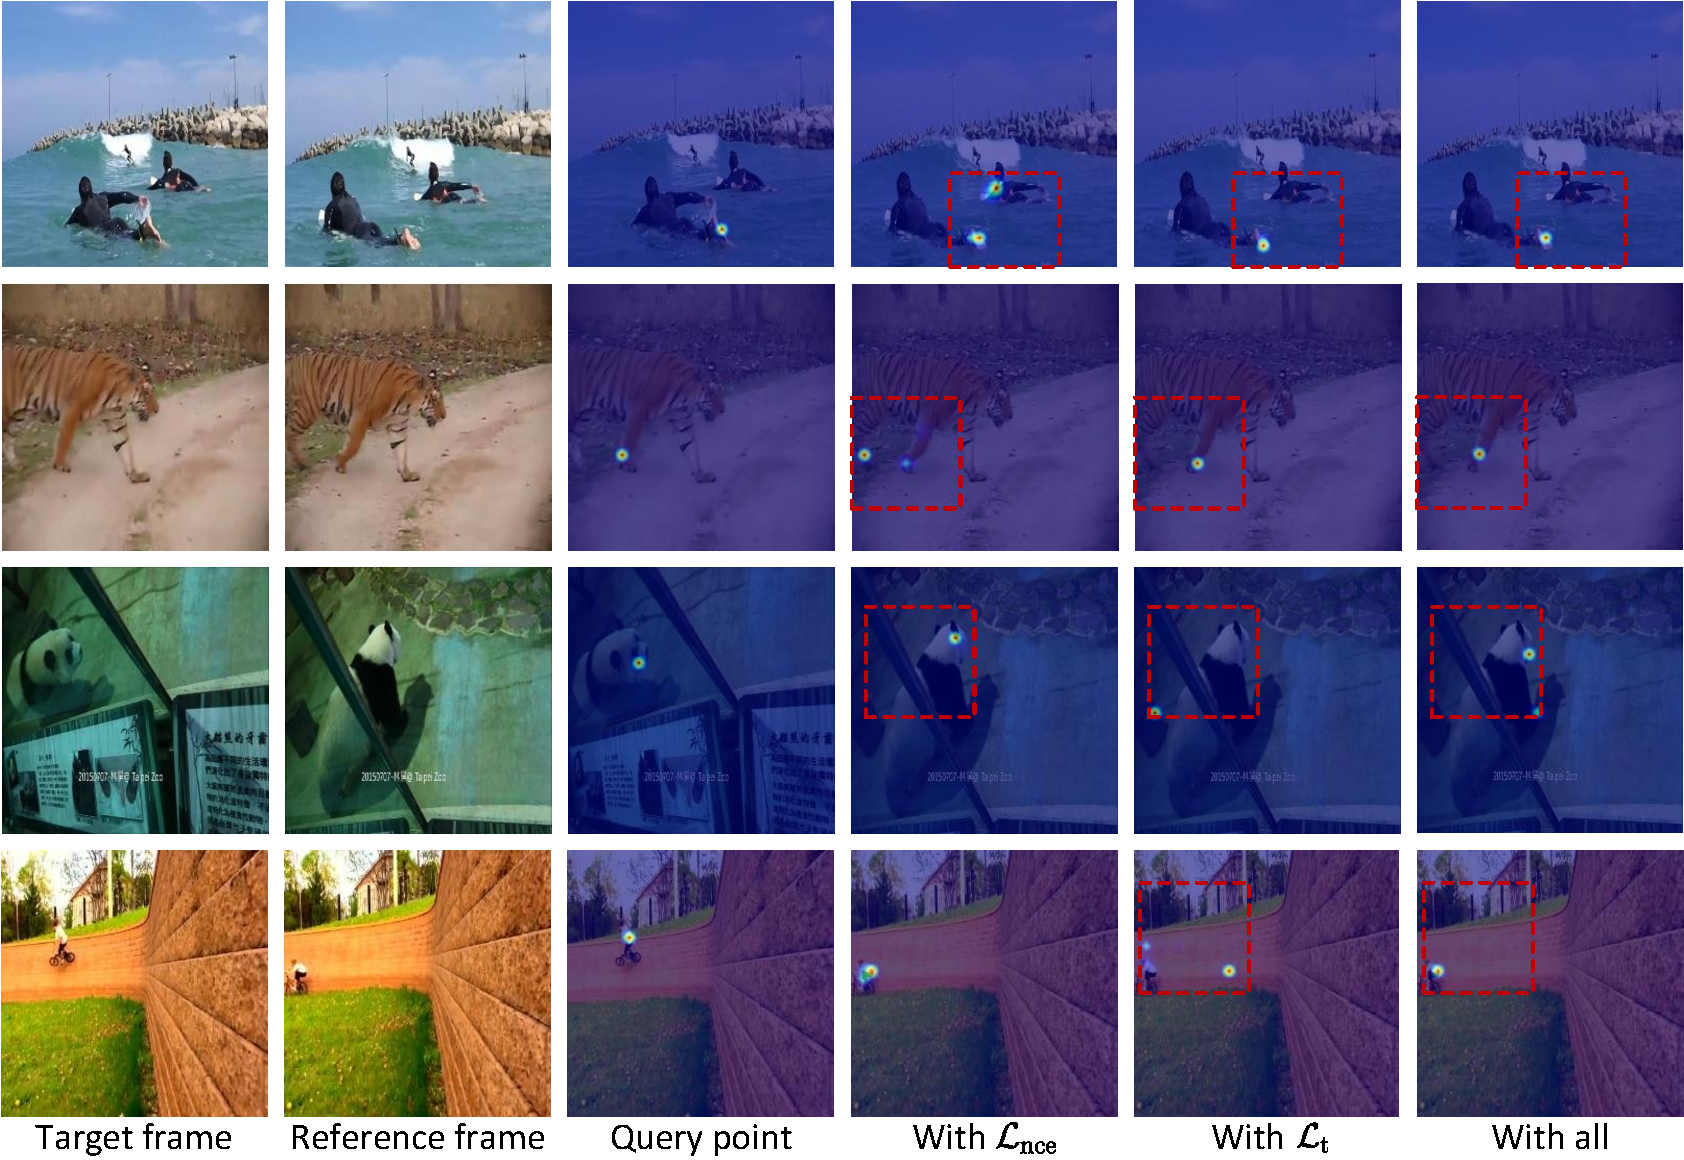
\includegraphics[width=1.0\textwidth]{figure/abalations/ablataions.pdf}}
  \caption{\small \textbf{Visualization of the ablation study.} Given a query point sampled in the target frame, we visualize the result of computing the local correlation  w.r.t. reference frame. The dashed line in red represents the range of computing correlation map w.r.t. query point. The reference frame is randomly sampled in the memory bank of inference strategy~\cite{jabri2020space}\cite{lai2020mast}\cite{xu2021rethinking}. }
  \label{fig:ablations}
  \vspace{-7mm}
\end{figure}

\textbf{Spatial feature learning.} We investigate the effect of training with each component in spatial feature learning. The results are shown in the last two rows of Table \ref{tab:ablations} (a). Note models are all first train on ImageNet and then switched to YouTube-VOS. With the help of the pre-training on ImageNet using contrastive loss, the performance of our method reaches 69.3\%. Moreover, the global correlation distillation loss $\mathcal{L}_{\mathrm{gc}}$ boosts up the performance from 69.3\% to 70.5\% by giving the ability of the model to capture object-level correspondence, which is closely related to object appearance modeling.
 
\textbf{Further exploitation of $\mathcal{L}_{\mathrm{gc}}$.}  Directly fine-tuning the model pre-trained with contrastive loss $\mathcal{L}_{\mathrm{nce}}$ will lead to a well-known phenomenon of catastrophic forgetting~\cite{li2017learning}, which is closely related to continual learning. To further verify the effectiveness of  $\mathcal{L}_{\mathrm{gc}}$, we exploit a general continual model LwF~\cite{li2017learning}  based on knowledge distillation apart from directly fine-tuning on video dataset. We modify the framework of LwF to adapt to the paradigm of self-supervised learning and adopt the framework of~\cite{xie2021detco} with ResNet-50 when training in the first step. The results are shown on Table \ref{tab:ablations} (b). All methods achieve better results attributed to the proposed temporal feature learning, while our method using $\mathcal{L}_{\mathrm{gc}}$ gets the best performance. 

\textbf{Further analysis.} 
We give a further analysis here based on the above experiments. On the one hand, temporal feature learning helps to learn the fine-grained correspondence related to motion estimation between frames, which is unable to accomplish by training an appearance model. As you can see in the second row of Figure \ref{fig:ablations}, the appearance model trained with $\mathcal{L}_{\mathrm{nce}}$ is misled by two patches at different locations (i.e. two feats of the tiger) which has a similar appearance, while the model trained with $\mathcal{L}_{\mathrm{t}}$ tends to learn a better temporal representation for fine-grained correspondence. However, in the last two rows of Figure \ref{fig:ablations}, the model trained with $\mathcal{L}_{\mathrm{t}}$ fails to capture temporal correspondence with a local correlation when facing severe temporal discontinuity, e.g., occlusions, appearance changes, large motion,  while the model trained with $\mathcal{L}_{\mathrm{nce}}$ is able to correct the mistakes by tracking the points based on the object appearance (see with $\mathcal{L}_{\mathrm{nce}}$ and with all).

\subsection{Comparison with State-of-the-art}

\begin{table*}[t]
	\centering
	\small
	\resizebox{0.99\textwidth}{!}{
		\setlength\tabcolsep{7.3pt}
		\renewcommand\arraystretch{1.05}
    % \renewcommand\thetable{2}
		\begin{tabular}{ccccccccc}
			\toprule
      & &  & & \multicolumn{2}{c}{Training Dataset} & & &  \\
      \cline{5-6}
			\multirow{-2}{*}{Method} & \multirow{-2}{*}{Sup.} & \multirow{-2}{*}{Backbone} & \multirow{-2}{*}{Stride} & Image & Video & \multirow{-2}{*}{$\mathcal{J}$\&$\mathcal{F}_m$ $\uparrow$} & \multirow{-2}{*}{$\mathcal{J}_m$ $\uparrow$}  &  \multirow{-2}{*}{$\mathcal{F}_m$ $\uparrow$}   \\  \hline
      MoCo~\cite{he2020momentum} & & ResNet-18 & 8 & ImageNet &-
			& 60.8 & 58.6  & 63.1  \\
      % DetCo & ResNet-18 & 8 & I &-
			% & 61.7 & 59.6  & 62.8  \\
      SimSiam~\cite{chen2021exploring} & & ResNet-18 & 8 & ImageNet &-
			& 62.0 & 60.0  & 64.0  \\
			Colorization~\cite{vondrick2018tracking} & & ResNet-18 & 8 & - & Kinetics
			& 34.0 & 34.6  & 32.7 \\
			CorrFlow~\cite{lai2019self} & & ResNet-18 & 8 & - & OxUvA
			& 50.3 & 48.4  & 52.2  \\
			MuG~\cite{lu2020learning} & & ResNet-18 &  8 & - & OxUvA
			& 54.3 & 52.6 & 56.1   \\
      UVC~\cite{li2019joint}  & & ResNet-18 & 8 & COCO & Kinetics
			& 59.5 & 57.7  & 61.3  \\
			ContrastCorr~\cite{wang2020contrastive} & & ResNet-18 & 8 & COCO  & TrackingNet
			& 63.0 & 60.5  & 65.5  \\
			VFS~\cite{xu2021rethinking}  & & ResNet-18 & 8 & - & Kinetics
			& 66.7 & 64.0  & 69.4  \\
      CRW~\cite{jabri2020space} & & ResNet-18 & 8 & - & Kinetics
			& 67.6 & 64.8  & 70.2  \\
			JSTG~\cite{zhao2021modelling} & & ResNet-18 & 8 & - & Kinetics
			& 68.7 & 65.8   & 71.6  \\
      DUL~\cite{araslanov2021dense} & & ResNet-18 & 8 & - & YTV
			& 69.3 & 67.1   & 71.6  \\
			% CLTC  & ResNet-18 & 8 & YT &(~-~, 5.58 hours)
			% & 70.3 & 67.9 & 78.2 & 72.6 & 83.7 \\
			\textbf{Ours} & & ResNet-18 & 8 & - & YTV
			& 69.0 & 66.4 & 71.7 \\
      \textbf{Ours} & & ResNet-18 & 8 & ImageNet & YTV
			& \textbf{70.5} & \textbf{67.8} & \textbf{73.2} \\
      \hline
      MAST~\cite{lai2020mast} & & ResNet-18 & 4 & - & YTV
			& 65.5 & 63.3  & 67.6  \\
      MAMP~\cite{miao2021self} & & ResNet-18 & 4 & - & YTV
			& 69.7 & 68.3   & 71.2  \\
      \textbf{Ours} & & ResNet-18 & 4 & - & YTV
			& 71.2  & 68.9 & 73.8 \\
      \textbf{Ours} & & ResNet-18 & 4 & ImageNet & YTV
			& \textbf{73.1} & \textbf{70.4} & \textbf{75.9} \\
			\hline
      MoCo~\cite{he2020momentum} & & ResNet-50 & 8 & ImageNet &-
			& 65.4 & 63.2  & 67.6  \\
      SimSiam~\cite{chen2021exploring} & & ResNet-50 & 8 & ImageNet &-
			& 66.3 & 64.5  & 68.2  \\
      % DetCo & ResNet-50 & 8 & I &-
			% & 66.5 & 64.7  & 68.4  \\
      TimeCycle~\cite{wang2019learning} & & ResNet-50 & 8 & - & VLOG
			& 48.7 & 46.4  & 50.0  \\
      UVC~\cite{li2019joint}  & & ResNet-50 & 8 & COCO & Kinetics
			& 56.3 & 54.5  & 58.1  \\
      % SeCo~\cite{yao2021seco} & & ResNet-50 & 8 & - & Kinetics
			% & 60.6 & 58.4  & 62.8  \\
      VINCE~\cite{gordon2020watching} & & ResNet-50 & 8 & - & Kinetics
			& 65.6 & 63.4  & 67.8  \\
      VFS~\cite{xu2021rethinking}  & & ResNet-50 & 8 & - & Kinetics
			& 68.9 & 66.5 & 71.3    \\
      \textbf{Ours} & & ResNet-50 & 8 & ImageNet & YTV
			& \textbf{71.3}  & \textbf{68.5} & \textbf{74.0}  \\
      \hline
      Supervised~\cite{he2016deep} &$\checkmark$ & ResNet-18 & 8 & ImageNet & -
			& 62.9 & 60.6  & 65.2  \\
      Supervised~\cite{he2016deep} & $\checkmark$& ResNet-50 & 8 & ImageNet &-
			& 66.0 & 63.7  & 68.4  \\
      OnAVOS~\cite{voigtlaender2017online} & $\checkmark$ & ResNet-38 & - & I + C + P & D
			& 65.4 & 61.6  & 69.1  \\
      OSVOS-S~\cite{maninis2018video}  & $\checkmark$ & VGG-16 & - & I + P & D
			& 68.0   & 64.7 & 71.3  \\
      FEELVOS~\cite{voigtlaender2019feelvos}  & $\checkmark$ & Xception-65 & - & I + C & D + YTV
			& 71.5   & 69.1 & 74.0  \\
			\bottomrule
		\end{tabular}
	}
	\captionsetup{font=footnotesize}
	\caption{\textbf{Quantitative results for video object segmentation on validation set of DAVIS-2017}~\cite{pont20172017}. We show results of state-of-the-art self-supervised methods and some supervised methods for comparison. We report the data size for self-supervised methods~(~total number/duration of image/video dataset~). ~I:ImageNet~\cite{deng2009imagenet}~(1.28m). ~C:COCO~\cite{lin2014microsoft}~(30k). ~O:OxUvA~\cite{valmadre2018long}~(14h). ~T:TrackingNet~\cite{muller2018trackingnet}~(300h). ~K:Kinetics~\cite{carreira2017quo}~(800h). ~V:VLOG~\cite{fouhey2018lifestyle}~(344h). ~YTV:YouTube-VOS~\cite{xu2018youtube}~(5h). ~D:DAVIS-2017~\cite{pont20172017}~(-). ~P:PASCAL-VOC~\cite{everingham2015pascal}~(-).}
	\label{table:sota}
	\vspace{-20pt}
\end{table*}


\textbf{Results for video object segmentation.}
We compare our method against previous self-supervised methods in Table \ref{table:sota}. For a fair comparison, we report both results of setting the stride of the encoder to 4 and 8. The results are all reported with layer $res_4$. Our method achieves state-of-the-art performance using both ResNet-18 and ResNet-50. For ResNet-18, our method with a stride of 8 achieves 70.5\%, making an absolute performance improvement by 1.2\% over all baselines using the same architecture. 
\begin{wraptable}{r}{8cm}
	\centering
	\small
	\resizebox{0.5\textwidth}{!}{
			\setlength\tabcolsep{3pt}
		\renewcommand\arraystretch{1.05}
		\begin{tabular}{ccccc}
            \toprule
		     & & \multicolumn{1}{c}{VIP} & \multicolumn{2}{c}{JHMDB} \\ \cline{3-5}
            \multirow{-2}{*}{Methods} & \multirow{-2}{*}{Sup.} & mIoU $\uparrow$   & PCK@0.1 $\uparrow$ & PCK@0.2 $\uparrow$
			\\ \midrule
      % ResNet-50 & $\checkmark$ & 39.5 & 59.2 & 78.3 \\
			TimeCycle~\cite{wang2019learning} &  & 28.9 & 57.3 & 78.1 \\
			UVC~\cite{li2019joint} &  & 34.1  & 58.6 & 79.6\\
			CRW~\cite{jabri2020space} &  & 38.6  & 59.3 & 80.3 \\
			ContrastCorr~\cite{wang2020contrastive} &  & 37.4  & 61.1 & 80.8 \\
			VFS~\cite{xu2021rethinking}  &  & 39.9  & 60.5 & 79.5\\
			CLTC~\cite{jeon2021mining} &  & 37.8  & 60.5 & 82.3\\
			JSTG~\cite{zhao2021modelling} &  & 40.2  & 61.4 & \textbf{85.3}\\
			\textbf{Ours} &  & \textbf{41.0} & \textbf{63.1} & 82.9\\
      \hline
      ResNet-18~\cite{he2016deep} & $\checkmark$ & 31.9 & 53.8 & 74.6 \\
      ATEN~\cite{zhou2018adaptive} & $\checkmark$ & 37.9 & - & -\\
      Thin-Slicing Net~\cite{song2017thin} & $\checkmark$ & - & 68.7 & 92.1\\
			\bottomrule
		\end{tabular}
	}
	\captionsetup{font=small}
	\caption{\textbf{Quantitative results for human part propagation and human pose tracking.} We show results of state-of-the-art self-supervised methods and some supervised methods for comparison.}
	\label{table:vip}
	\vspace{-9pt}
\end{wraptable}
Benefiting from exploiting more fine-grained supervision for temporal feature learning by setting the stride of the encoder to 4, the performance of our method reaches 73.1\%, leading to a performance gain of 3.4\% over MAMP~\cite{miao2021self}, which consistently verify the idea of our methods.
For ResNet-50, our method still outperforms VFS~\cite{xu2021rethinking} by 2.4\%. It is worth noting that \cite{jabri2020space}\cite{li2019joint}\cite{wang2020contrastive}\cite{xu2021rethinking}\cite{zhao2021modelling} are all pre-trained on large-scale video datasets, i.e., Kinetics~\cite{carreira2017quo}, TrackingNet~\cite{muller2018trackingnet}, while our method adopt a small video dataset plus an image dataset which has a much smaller data size than video.  Besides, the performance reaches 69.0\%/71.2\% when training only on YouTube-VOS, which is impressive.  More remarkably, Our method even outperforms some task-specific fully-supervised algorithms~\cite{maninis2018video}\cite{voigtlaender2017online}\cite{voigtlaender2019feelvos}.



\textbf{Results for human part propagation.} Next, we evaluate our method for human part tracking. Experiments are conducted on the validation set of VIP~\cite{zhou2018adaptive}, which consists of 50 videos with 19 human semantic part, requiring more precise matching than DAVIS-2017~\cite{pont20172017}. Following~\cite{zhou2018adaptive}, we adopt mean intersection-over-union (mIoU) as our evaluation metric and resize the video frames to 560 $\times$ 560. All models except TimeCycle~\cite{wang2019learning} are set to ResNet-18 with a stride of 8 for a fair comparison. The results are shown in Table \ref{table:vip}. Our method achieves state-of-the-art performance, surpassing previous state-of-the-art by 0.8\%. Notably, our model outperforms ATEN~\cite{zhou2018adaptive} which is specifically designed for this task using human annotations. Figure \ref{fig:quan} (b) depicts some visualization results on several representative videos.


\textbf{Results for human pose tracking.} We then make a performance comparison on the downstream task of human pose tracking. We conduct the experiments on the validation of JHMDB~\cite{jhuang2013towards} which has 268 videos. The annotations consist of 15 body joints for each person. The probability of correct keypoint~\cite{yang2012articulated} is utilized here to examine the accuracy  with different thresholds. Following the evaluation protocol of~\cite{jabri2020space}\cite{li2019joint}, we resize the video frames to 320 $\times$ 320. The results in Table \ref{table:vip} show a consistent performance gain over previous methods, which successfully demonstrates the transferability of our method to different downstream tasks. The visualization results in Figure \ref{fig:quan}~(c) show the robustness of our approach to various challenges.


\begin{figure}[!tb]
  \centering
  {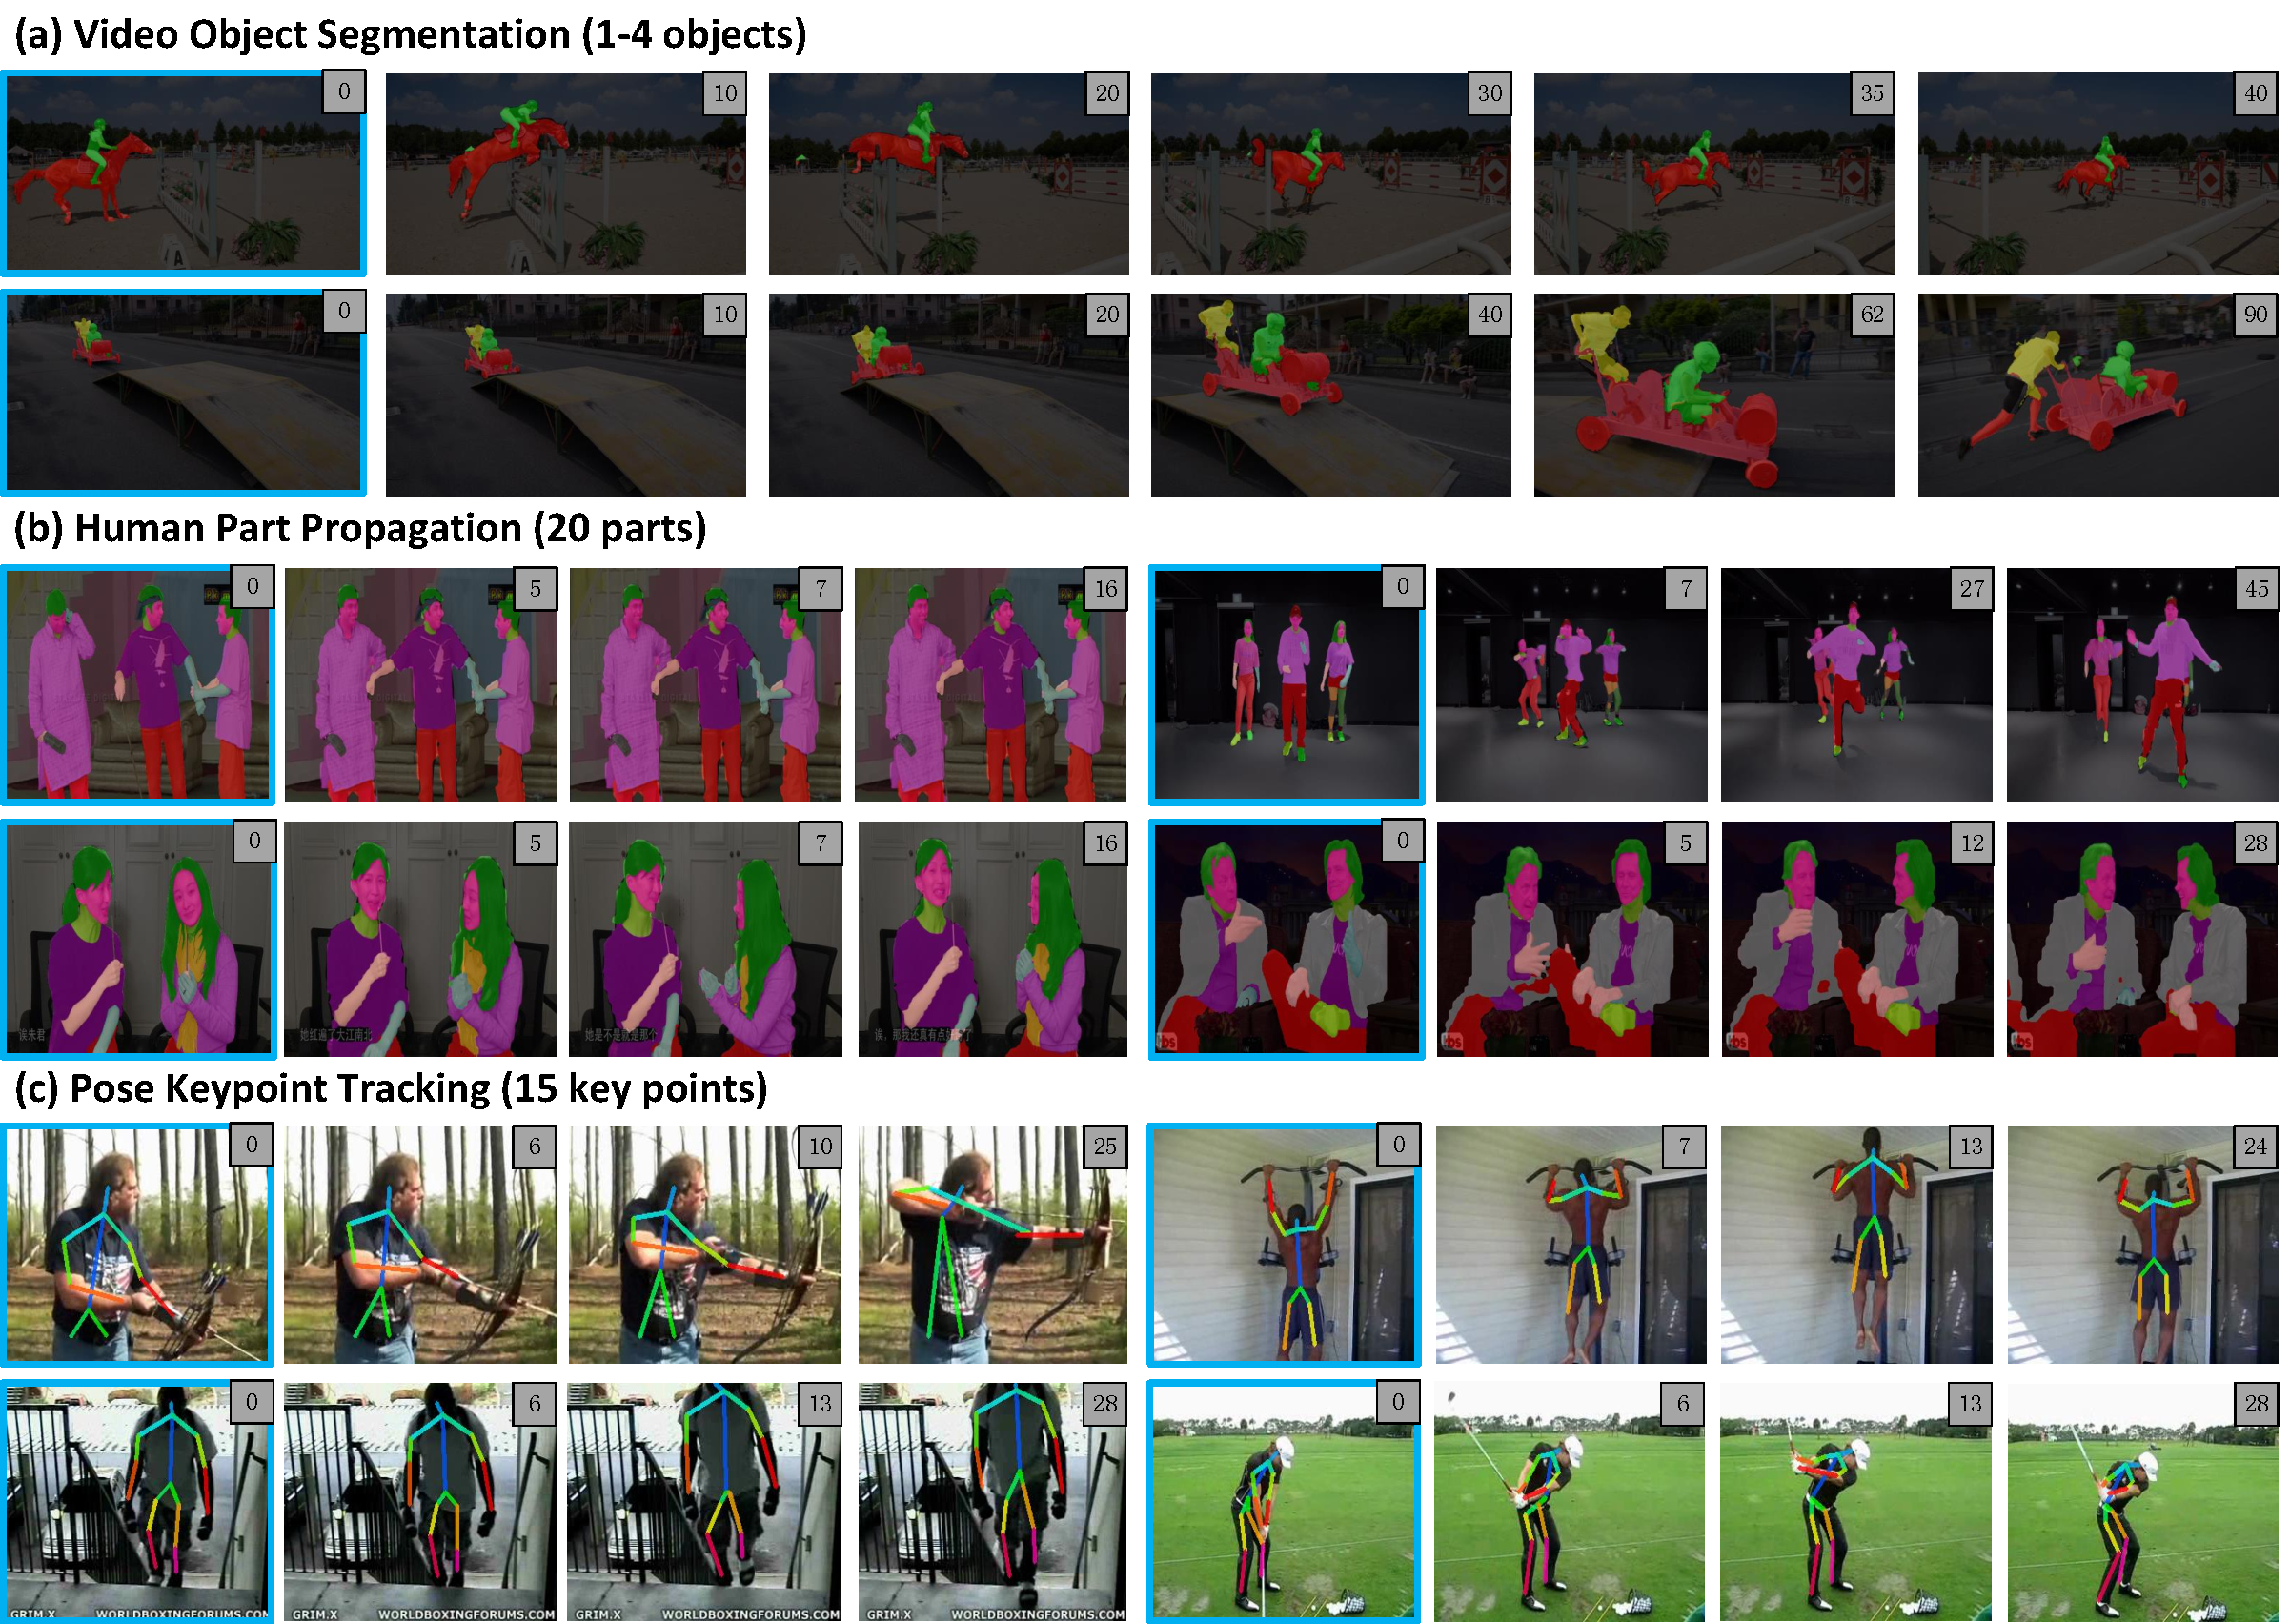
\includegraphics[width=1.0\textwidth]{figure/quantitative_results/quan.pdf}}
  \caption{\small Qualitative results for label propagation. Given the first frame with different annotations highlighted with a blue outline, we propagate it to the current frame without fine-tuning. (a) Video object segmentation on DAVIS-2017~\cite{pont20172017}. (b) Human part propagation on VIP~\cite{zhou2018adaptive}. (c) Pose keypoint tracking on JHMDB~\cite{jhuang2013towards}. }
  \label{fig:quan}
  \vspace{-6mm}
\end{figure}

\section{Conclusions}
In this work,  we propose a new spatial-then-temporal pretext task for training data-efficient self-supervised learning for video correspondence.  We first train a model using contrastive loss on ImageNet, and then perform temporal feature learning with the objective of frame reconstruction on a small video dataset. To retain appearance sensitivity, the global correlation distillation is conducted at the coarse pyramid level. At the same time, we regard the local correlation map computed at fine-grained pyramid level as pseudo labels to address the problem of temporal discontinuity.  Extensive experiments on a variety of downstream tasks validate our method. We hope our method can provide a new perspective for self-supervised video correspondence learning. 


\medskip


{
\small

\bibliographystyle{abbrvnat}
\bibliography{neurips_2022}
}
% {\small
% \bibliographystyle{ieee_fullname}
% \bibliography{neurips_2022}
% }


%%%%%%%%%%%%%%%%%%%%%%%%%%%%%%%%%%%%%%%%%%%%%%%%%%%%%%%%%%%%
\section*{Checklist}


%%% BEGIN INSTRUCTIONS %%%
The checklist follows the references.  Please
read the checklist guidelines carefully for information on how to answer these
questions.  For each question, change the default \answerTODO{} to \answerYes{},
\answerNo{}, or \answerNA{}.  You are strongly encouraged to include a {\bf
justification to your answer}, either by referencing the appropriate section of
your paper or providing a brief inline description.  For example:
\begin{itemize}
  \item Did you include the license to the code and datasets? \answerYes
  \item Did you include the license to the code and datasets? \answerNo{The code and the data are proprietary.}
  \item Did you include the license to the code and datasets? \answerNA{}
\end{itemize}
Please do not modify the questions and only use the provided macros for your
answers.  Note that the Checklist section does not count towards the page
limit.  In your paper, please delete this instructions block and only keep the
Checklist section heading above along with the questions/answers below.
%%% END INSTRUCTIONS %%%


\begin{enumerate}


\item For all authors...
\begin{enumerate}
  \item Do the main claims made in the abstract and introduction accurately reflect the paper's contributions and scope?
    \answerTODO{}
  \item Did you describe the limitations of your work?
    \answerTODO{}
  \item Did you discuss any potential negative societal impacts of your work?
    \answerTODO{}
  \item Have you read the ethics review guidelines and ensured that your paper conforms to them?
    \answerTODO{}
\end{enumerate}


\item If you are including theoretical results...
\begin{enumerate}
  \item Did you state the full set of assumptions of all theoretical results?
    \answerTODO{}
        \item Did you include complete proofs of all theoretical results?
    \answerTODO{}
\end{enumerate}


\item If you ran experiments...
\begin{enumerate}
  \item Did you include the code, data, and instructions needed to reproduce the main experimental results (either in the supplemental material or as a URL)?
    \answerTODO{}
  \item Did you specify all the training details (e.g., data splits, hyperparameters, how they were chosen)?
    \answerTODO{}
        \item Did you report error bars (e.g., with respect to the random seed after running experiments multiple times)?
    \answerTODO{}
        \item Did you include the total amount of compute and the type of resources used (e.g., type of GPUs, internal cluster, or cloud provider)?
    \answerTODO{}
\end{enumerate}


\item If you are using existing assets (e.g., code, data, models) or curating/releasing new assets...
\begin{enumerate}
  \item If your work uses existing assets, did you cite the creators?
    \answerTODO{}
  \item Did you mention the license of the assets?
    \answerTODO{}
  \item Did you include any new assets either in the supplemental material or as a URL?
    \answerTODO{}
  \item Did you discuss whether and how consent was obtained from people whose data you're using/curating?
    \answerTODO{}
  \item Did you discuss whether the data you are using/curating contains personally identifiable information or offensive content?
    \answerTODO{}
\end{enumerate}


\item If you used crowdsourcing or conducted research with human subjects...
\begin{enumerate}
  \item Did you include the full text of instructions given to participants and screenshots, if applicable?
    \answerTODO{}
  \item Did you describe any potential participant risks, with links to Institutional Review Board (IRB) approvals, if applicable?
    \answerTODO{}
  \item Did you include the estimated hourly wage paid to participants and the total amount spent on participant compensation?
    \answerTODO{}
\end{enumerate}


\end{enumerate}


%%%%%%%%%%%%%%%%%%%%%%%%%%%%%%%%%%%%%%%%%%%%%%%%%%%%%%%%%%%%


\appendix





\end{document}